\section{Sprint 6}

Il progetto di riferimento per questo sprint è it.unibo.ddrsystem6.

OBIETTIVO: creazione di un sistema con un robot che  una volta ricevuto il comando di "start", inizi a esplorare autonomamente la stanza in cui si trova solo se la temperatura della stanza è al di sotto di una certa soglia (R-tempOk). Una volta iniziata la fase di esplorazione, non appena la temperatura della stanza supera la soglia il robot si deve fermare. 
Durante l'esplorazione, se il robot riceve il comando di backHome (R-backHome), il robot deve sospendere l'esplorazione e tornare alla base.
Durante l'esplorazione il robot deve anche far blinkare un led (R-blinkLed).

Work plan:
\begin{enumerate}
\item definizione di una strategia con cui poter controllare la temperatura della stanza;
\item gestione del cambio di temperatura nel caso in cui essa superi una certa soglia;
\item gestione del messaggio di "backHome";
\item gestione del blinking del led posto sul robot durante la fase di esplorazione.
\end{enumerate}

\subsection{Analisi dei requisiti}

\textbf{Cosa si intende per variazione della temperatura della stanza?}
Per variazione della temperatura della stanza si intende un cambiamento significativo di essa che la porti ad assumere un valore superiore o inferiore ad una soglia fissata. 

\textbf{Cosa si intende per blinking del led?}\\
Per blinking del led si intende, nel caso del robot fisico, l'accensione ad intermittenza un led posto su di esso. Nel caso del robot simulato tale comportamento è simulato con una stampa su console ("blinking").

\subsection{Analisi del problema}

\textbf{Come è possibile gestire la variazione della temperatura della stanza?}\\

La variazione è gestita utilizzando due bottoni "OK" e "TOOHIGH". Quando il primo viene premuto significa che la temperatura è al di sotto di una certa soglia e non sono state rilevate variazioni particolarmente significative (temperatura accettabile). Invece, quando viene premuto il secondo bottone significa che vi è stata una variazione della temperatura tale da comportare l'arresto dell'esplorazione (temperatura alta).
Ad inizio esplorazione si ipotizza che la temperatura della stanza sia corretta. Una volta che  il bottone "TOOHIGH" viene premuto, il robot deve sospendersi in attesa che la temperatura ritorni nella norma (premendo il bottone "OK") e che l'operatore ridia il comando di "start".

\textbf{Come è possibile gestire il comando di "backHome"?}\\
L'esplorazione del robot è suddivisa nel raggiungimento di diversi goal. (i.e. (0,0)(1,1)(2,2)...) Quando l'operatore spinge il bottone di "backHome" è sufficiente indicare al robot che il goal da perseguire corrisponde alla propria base (0,0) e una volta che lo ha raggiunto aspettare che l'operatore ridia il comando di "start" per riprendere l'esplorazione. 

\textbf{Come è possibile gestire il blinking del led?}\\
Il task del blinking, pur essendo una funzionalità a parte rispetto a quella di esplorazione, deve comunque essere gestito in contemporanea rispetto a quest'ultimo. Quindi potrebbe risultare utile incapsulare tale comportamento in un'entità separata


\subsection{Model}

Per quanto riguarda la gestione della temperatura, è necessario modificare il behaviour del QKActor robotmind. Robotmind, sia prima di iniziare l'esplorazione, sia mentre questa è in corso, controlla se nel sistema si verifica un evento di "temperatureTooHigh". Nel primo caso, se ciò accade, il robot dovrà aspettare che si verifichi l'evento di "temperatureOk" e un comando di "start" prima di dare il via all'esplorazione. Nel secondo caso, il robot, arresta momentaneamente l'esplorazione sospendendo il piano che stava svolgendo, ponendosi prima in attesa dell'evento "temperatureOk" e poi del comando di "start" che gli consenta di riprenderla. Nel caso l'evento di "temperatureOk" non arrivi mai, il robot rimarrà fermo nella sua posizione attuale.
Il listing \ref{lst:robotmind_ddr_sys_6_temp} riporta il codice per gestire la logica applicativa della temperatura.


\begin{lstlisting}[backgroundcolor=\color{white}, label={lst:robotmind_ddr_sys_6_temp}, caption={Codice di QActor robotmind in ddrSystem6} ]
Event temperatureTooHigh: temperatureTooHigh

QActor robotmind context robotMindCtx {

	State waitForStart {
		...
	}

	Transition t0  whenEvent startCmd  -> startExploration
				   whenEvent temperatureTooHigh  -> waitForTemperatureOk
   
    ...
    
    State startExploration {
    	...
		
	} 

	Transition t1 whenEvent temperatureTooHigh -> waitForTemperatureOk
	              ...

    State backHome {
		   println("========== robotmind: backHome ==========")	  
		  forward planexecutor -m stopPlan: stopPlan
		  run itunibo.planner.plannerUtil.setGoal(0,0)
		  forward planexecutor -m doPlan : doPlan(0,0)   
	}
	Transition t2 whenEvent temperatureTooHigh  -> waitForTemperatureOk
	              ...
	              
	State handleStartAfterBackHome { }
	Transition t0  whenEvent temperatureTooHigh  -> waitForTemperatureOk
	                ...
	
	              
\end{lstlisting}

Quando l'operatore clicca il pulsante "backHome" sulla propria console tale evento viene catturato dal QKActor robotmind quando quest'ultimo si trova nello stato "startExploration". Una volta catturato tale evento prima di tutto interrompe il piano attualmente in esecuzione e poi imposta il nuovo goal a (0,0) in modo da tornare alla base. Una volta terminato il goal, robotmind, si mette in attesa dello "start". Nel caso in cui, durante tutto il procedimento, dovesse percepire l'evento di "stopCmd" oppure di "temperatureTooHigh", sospenderà l'esecuzione del compito per attendere gli opportuni comandi prima di ricominciare.
Il listing \ref{lst:backHome-ddr-sys-6} riporta il codice per gestire la logica applicativa del backHome.

\begin{lstlisting}[backgroundcolor=\color{white}, label={lst:backHome-ddr-sys-6}, caption={"Codice di robotmind per la gestione del backHome"}]

State startExploration {... } 

	Transition t1 ...
	             whenEvent backHomeCmd -> backHome

	State backHome {
		  forward planexecutor -m stopPlan: stopPlan
		  run itunibo.planner.plannerUtil.setGoal(0,0)
		  forward planexecutor -m doPlan : doPlan(0,0)   
	}
	Transition t2 whenMsg planOk -> handleStartAfterBackHome 
			      whenMsg planFail -> backHome
			      whenEvent stopCmd -> waitForStart
			      whenEvent temperatureTooHigh  -> waitForTemperatureOk
	
	State handleStartAfterBackHome {	}
	Transition t0  whenEvent startCmd  -> startExploration
				   whenEvent temperatureTooHigh  -> waitForTemperatureOk

\end{lstlisting}



Dal momento che si è individuato il compito del blinking del led come task separato rispetto a quello dell'esplorazione, ma che deve comunque essere svolto contemporaneamente, si è deciso di assegnare la gestione di tale compito ad un QKActor diverso da robotmind, denominato blinkinghandler. Tale attore, ogni volta che riceve il messaggio di "startBlinking" dovrà comunicare al robotactuator di iniziare il compito del blinking, e quando riceve il messaggio di stopBlinking, dovrà comunicare al robotactuator di terminarlo.
Dati i requisiti, la robotmind indicherà al blinkinghandler di avviare tale task non appena inizia la fase di esplorazione e di terminarlo quando viene individuata la valigia con la bomba.
Il listing \ref{lst:blinking-ddr-sys-6} riporta il codice per gestire la logica applicativa del blinkingLed.


\begin{lstlisting}[backgroundcolor=\color{white}, label={lst:blinking-ddr-sys-6}, caption={"Codice di blinkinghandler in ddrSystem6"}]

QActor blinkinghandler context robotMindCtx {
	
		State s0 initial {		}
		Transition t0 whenMsg startBlinking -> sendBlinkingMsg
		
		State sendBlinkingMsg{
			println("========== blinking ==========")
			forward robotactuator -m robotCmd : robotCmd (blinking)
		}
		Transition t1 whenMsg stopBlinking -> stopBlinking
		
		State stopBlinking{
			println("========== stop blinking ==========")
			forward robotactuator -m robotCmd : robotCmd (stopBlinking)
		}		
		Goto s0
}
\end{lstlisting}


In questo sistema si è revisionata anche la strategia di esplorazione: ora il robot, terminata una "chiocciola", prima di passare a quella successiva, esplora tutte le caselle a "0" presenti, senza esplorarle tutte una volta trovate le pareti. Questa nuova strategia permette di trovare un'eventuale bomba "as soon as possible".


L'architettura del sistema è riportata in \cref{fig:arch_logica_6}.

\begin{figure}[H]
  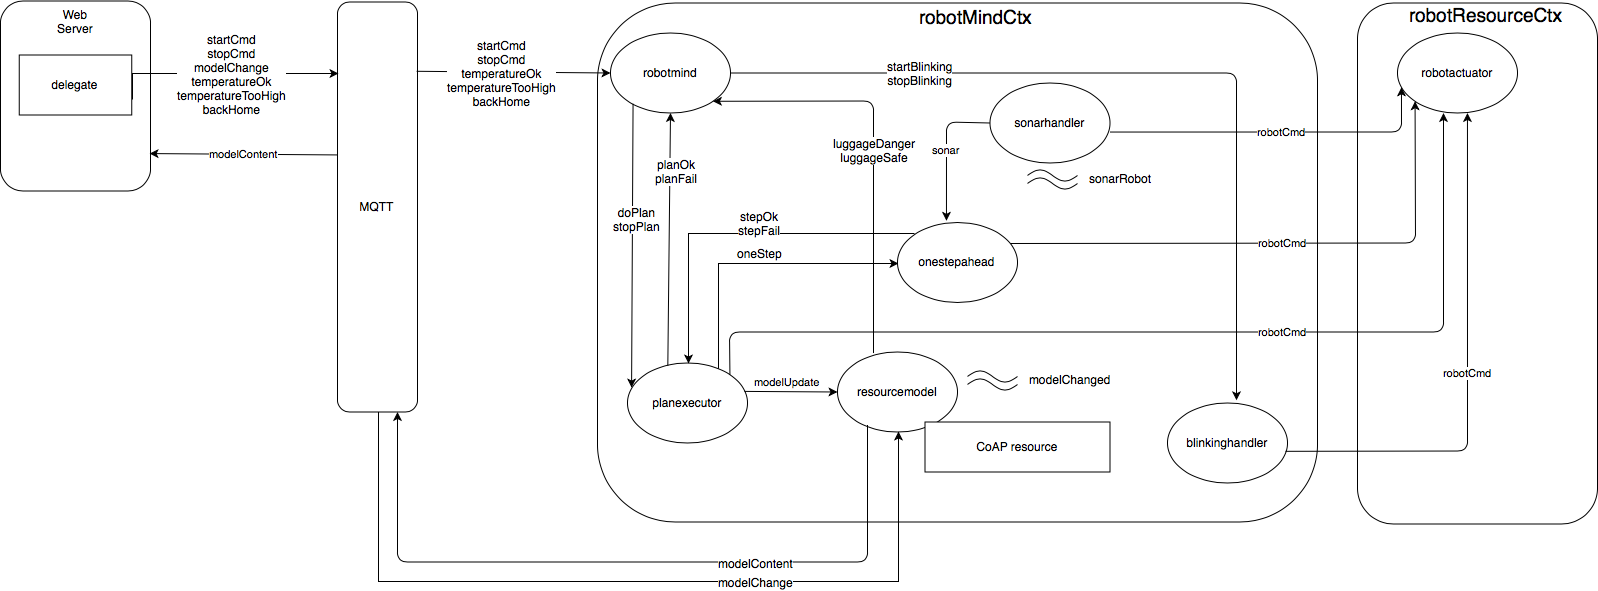
\includegraphics[width=1.7\textwidth, angle=270]{img/sprint6/arch_logica_6.png}
  \caption{L'architettura del sistema.}
  \label{fig:arch_logica_6}
\end{figure}



\subsection{Test plan}

Verificare il corretto funzionamento del sistema:

\begin{itemize}
\item verificare che il robot, una volta percepito l'evento di "temperatureTooHigh", sospenda l'esplorazione;
\item verificare che il robot, una volta sospesa l'esplorazione a seguito dell'evento "temperatureTooHigh" la riprenda solo una volta percepiti in ordine gli eventi "temperatureOk" e "startCmd":
\item verificare che il robot, una volta ripresa l'esplorazione dopo averla interrotta a causa della temperatura oltre la soglia, reimposti il goal corretto, ossia quello che stava svolgendo prima di fermarsi;
\item verificare che il robot, una volta percepito l'evento di "backHome", imposti il goal a (0,0);
\item verificare che il robot, una volta tornato alla base poiché ricevuto il comando di "backHome", si metta in attesa del comando di "start";
\item verificare che il robot, una volta ripresa la fase di esplorazione, dopo averla interrotta a causa del comando di "backHome", reimposti il goal corretto: quello che stava svolgendo prima di impostare (0,0);
\item verificare che il robot, non appena inizia la fase di esplorazione, avvi anche il blinking del led sul robot;
\item verificare che il robot, non appena termina la fase di esplorazione (o perché ha trovato la bomba o perché ha esplorato tutte le celle della stanza), termini anche il compito del blinking del led;
\end{itemize}{}
